\documentclass[12pt]{article}
\usepackage{amsmath,amsfonts,amsthm,amssymb,graphicx,authblk}
\usepackage[font={footnotesize,singlespacing},labelfont=bf]{caption}
\usepackage{blkarray, bm} 
\usepackage{float,afterpage}
\usepackage[running,mathlines]{lineno}

\usepackage{xr}
\externaldocument[ms-]{BetterGrowthModeling_r1_appendices}

\usepackage[verbose,letterpaper,tmargin=2.54cm,bmargin=2.54cm,lmargin=2.54cm,rmargin=2.54cm]{geometry}
\usepackage[authoryear,sort]{natbib}
\usepackage[dvipsnames]{xcolor}
\usepackage{hyperref}

\usepackage[compact,small]{titlesec}
\usepackage[moderate]{savetrees}

\usepackage{enumitem}
\setlist{topsep=.1em,itemsep=-0.2em,leftmargin=0.75cm}

\setlength{\parindent}{0.35in}
% \usepackage[sc]{mathpazo} %Like Palatino with extensive math support
\usepackage[scale=1]{newtxtext,newtxmath} 

\usepackage{siunitx}

\usepackage[nodisplayskipstretch]{setspace} 

% Coloring of R code listings
\usepackage[formats]{listings}
\usepackage{color}
\definecolor{mygreen}{rgb}{0.1,0.5,0.1}
\definecolor{mygray}{rgb}{0.5,0.5,0.5}
\definecolor{mymauve}{rgb}{0.58,0,0.82}
\definecolor{mygrey}{rgb}{0.3,0.3,0.1}
\lstset{
language=R,
otherkeywords={data.frame},
basicstyle=\normalsize\ttfamily, 
commentstyle=\normalsize\ttfamily,
keywordstyle=\normalsize\ttfamily,
stringstyle=\color{mymauve}, 
commentstyle=\color{mygreen},
keywordstyle=\color{blue},
showstringspaces=false, xleftmargin=2.5ex,
columns=flexible,
literate={~}{{$\sim \; \; $}}1,
alsodigit={\.,\_},
deletekeywords={on,by,data,R,Q,mean,var,sd,log,family,na,options,q,weights,effects,matrix,nrow,ncol,wt,fix,distance},
}
\lstset{escapeinside={(*}{*)}} 

\lstdefineformat{Rpretty}{
	; = \space,
	\, = [\ \,\]]\string\space,
	<- = [\ ]\space\string\space,
	\= = [\ ]\space\string\space}


%\usepackage{lineno}
\renewcommand{\refname}{Literature Cited}
\renewcommand{\floatpagefraction}{0.9}
\renewcommand{\topfraction}{0.99}
\renewcommand{\textfraction}{0.05}

\clubpenalty = 10000
\widowpenalty = 10000

\sloppy 

\usepackage{ifpdf}
\ifpdf
\DeclareGraphicsExtensions{.pdf,.png,.jpg}
\usepackage{epstopdf}
\else
\DeclareGraphicsExtensions{.eps}
\fi

% commands for commenting
\newcommand{\tom}[2]{{\color{red}{#1}}\footnote{\textit{\color{red}{#2}}}}
\newcommand{\steve}[2]{{\color{blue}{#1}}\footnote{\textit{\color{blue}{#2}}}}
\newcommand{\revise}[1]{{\color{Mahogany}{#1}}}
%%%%%%%%%%%%%%%%%%%%%%%%%%%%%%%%%%%%%%%%%%%%% 
%%% Just for commenting
%%%%%%%%%%%%%%%%%%%%%%%%%%%%%%%%%%%%%%%%%%%%
\usepackage[dvipsnames]{xcolor}
\newcommand{\comment}{\textcolor{blue}}
\newcommand{\new}{\textcolor{red}}

\newcommand{\be}{\begin{equation}}
\newcommand{\ee}{\end{equation}}

\newcommand{\red}{\textcolor{red}}


\title{My, how you've grown: \\ A practical guide to modeling size transitions \\ for Integral Projection Model (IPM) applications}

\author[a]{Tom E.X. Miller\thanks{Corresponding author. Department of BioSciences, Rice University,
Houston, TX 77005-1827. Email: tom.miller@rice.edu Phone: 713-348-4218}}
\author[b]{Stephen P. Ellner}
\affil[a]{Department of BioSciences, Rice University, Houston, TX USA} 
\affil[b]{Department of Ecology \& Evolutionary Biology, Cornell University, Ithaca, NY USA} 
\date{}
\renewcommand\Authands{ and }

\sloppy

\begin{document}

\begin{spacing}{1.7} 

\maketitle
\bigskip 
\noindent\textbf{Submitted to:} \textit{Ecology} (Statistical Report)

%alphabetical order not exceeding eight words or short phrases
\bigskip
\noindent\textbf{Keywords}: demography; growth; integral projection model; kurtosis; skewness

\bigskip 
\noindent\textbf{Open Research Statement:} Data are already published and publicly available, with those items properly cited in this submission. Three data sets are cited as data packages \citep{cactusdata, shrubdata, winfield2013pikegrowth}. Two other data sets, as well as all of our code, are available in \cite{zenodo3924640}.  

\newpage
%\linenumbers
%%%%%%%%%%%%%%%%%%%%%%%%%%%%%%%%%%%%%%%%%%%%%%%%%%%%%%%%%%%%%%%%%%%%%%
%\spacing{1.6} 
%350 word limit on abstract, must be numbered 1-4

%TC:ignore

\end{spacing} 
\begin{spacing}{1.9}
\linenumbers
\noindent 
\textbf{\large{Abstract}} 
% ESA Statistical Report limit: 200 words

Integral Projection Models (IPMs) are widely used for studying continuously size-structured populations. 
IPMs require a growth sub-model that describes the probability of future size conditional on current size and any covariates. 
Most IPM studies assume that this distribution is Gaussian, despite calls for non-Gaussian models that accommodate skewness and excess kurtosis. 
We provide a general workflow for accommodating non-Gaussian growth patterns while retaining important covariates and random effects. 
Our approach emphasizes visual diagnostics from pilot Gaussian models and quantile-based metrics of skewness and kurtosis that guide selection of a non-Gaussian alternative, if necessary. 
Across five case studies, skewness and excess kurtosis were common features of growth data and non-Gaussian models consistently generated simulated data that were more consistent with real data than pilot Gaussian models. 
However, effects of ``improved'' growth modeling on IPM results were moderate to weak, and differed in direction or magnitude between different outputs from the same model. 
Using tools not available when IPMs were first developed, it is now possible to fit non-Gaussian models to growth data without sacrificing ecological complexity. 
Doing so, as guided by careful interrogation of the data, will result in models that better represent the populations for which they are intended. 

%TC:endignore

\newpage
\section{Introduction}

Structured demographic models -- matrix and integral projection models (MPMs and IPMs) -- are powerful tools for data-driven modeling of population and community dynamics. 
In contrast to MPMs for populations with discrete structure (life stage, age class, etc.), IPMs \citep{easterling2000size} accommodate populations structured by continuous state variables, most commonly size. 
A related innovation of the IPM framework is its emphasis on regression-based modeling for parameter estimation, which 
often carries important advantages for making the most of hard-won data \citep{ellner2022critical}.  

A standard workflow allows ecologists to assemble an IPM from data using familiar regression tools to describe growth, survival, reproduction, and other demographic transitions as functions of size \citep{Coulson:2012fk,ellner-etal-2016}. 
The relative ease of regression analyses, accommodating covariates (e.g., environmental factors, experimental treatments) and complex variance structures (e.g., random effects, correlated errors), has facilitated a growing IPM literature that examines how biotic or abiotic factors affect population dynamics \citep[e.g.,][]{ozgul2010coupled,louthan2022climate} and explores the consequences of demographic heterogeneity associated with spatial, temporal, and individual variation \citep[e.g.,][]{crone2016contrasting,compagnoni2016effect,plard2018sex}. 
The vital rate regressions (or ``sub-models'') are the bridge between the individual-level data and the population-level model and its predictions; it is important to get those right.

Compared to other vital rates, growth is special. 
The survival and reproduction sub-models only need to provide a single predicted value as functions of size (we use ``size'' as the name for whatever continuous variable defines the population structure).   
But the growth model must specify the full probability distribution of subsequent size conditional on initial size, defining the  
growth `kernel' $G(z',z)$ that gives the probability density of future size $z'$ at time $t+1$ conditional on current size $z$ at time $t$. 
Whenever survival and reproduction are size-dependent, the entire distribution of size transitions can strongly influence IPM predictions because it governs how frequently size changes are much greater or much lower than average. 

Easterling et al. \citeyear{easterling2000size} provided the original template for modeling size transitions in IPMs. 
They first tried simple linear regression, assuming Normally distributed size changes with constant variance. 
Because the residuals from this regression exhibited non-constant variance, they used a two-step approach to estimate the size-dependence in mean squared residuals (better options soon became available, such as the \texttt{lme} function in R). 
However, even after accounting for non-constant variance, growth data may still be non-Normal.  
Size transitions are often skewed such that large decreases are more common than large increases \citep{peterson2019improving,salguero2010keeping}, or vice versa \citep{stubberud2019effects}.
Size transitions may also exhibit excess kurtosis (``fat tails''), where extreme growth or shrinkage is more common than predicted by the tails of the Normal distribution \citep{herault2011functional}. 

The observation that the Normal (or Gaussian) distribution may poorly describe size transitions in real organisms has been made before,  
and several studies have emphasized that alternative distributions should be explored \citep{easterling2000size,peterson2019improving,rees2014building,williams2012avoiding}. 
For example, Peterson et al. \citeyear{peterson2019improving} showed that skewness in size transitions could be modeled through beta regression on transformed data (for reasons we describe below, this approach also has some drawbacks),
or by fitting a skewed Normal distribution. 
They showed that incorporating skew could have important consequences for model-based inferences, and concluded that ``testing of alternative distributions for growth$\ldots$ [should] become standard in the construction of size-structured population models.''
Nonetheless, default use of Gaussian growth distributions (often with non-constant variance) remains the standard practice. 
The general state-of-the-art in the literature appears to remain where it was 20 or so years ago, using the default Gaussian model without examining critically whether or not it actually describes the data well.  
We are guilty of this, ourselves. 

The persistence of Gaussian growth models is understandable. 
%The Gaussian is the maximum entropy distribution for real-valued observations with finite variance. 
% There is a long tradition of statistical modeling built on the assumption of normally distributed residuals with constant variance.
Popular pacakges such as lme4 \citep{bates2007lme4}, mgcv \citep{wood-2017}, and MCMCglmm \citep{hadfield2010mcmc} make it easy to fit growth models with potentially complex fixed- and random-effect structures, but the possible distributions of continuous responses are limited, and default to Gaussian. 
Abandoning these convenient tools for the sake of more flexible growth modeling means, it may seem, sacrificing the flexibility to model diverse sources of demographic variation, some of which may be the motivation driving the study in the first place.

Our goal here is to present and illustrate a practical ``recipe'' that moves growth modeling past the standards set over 20 years ago. 
Using software tools that are now readily accessible, ecologists can escape the apparent trade-off between realistically modeling non-Gaussian size transitions and flexibly including multiple covariates and random effects.\footnote{Our statements about software availability are based on what current software reliably delivers in our personal experience, not on what they promise.} 
As with any recipe, users may need to make substitutions or add ingredients to suit their needs. 
We emphasize graphical diagnostics for developing and evaluating growth models, rather than a process centered on statistical tests or model selection. 
Through empirical case studies we demonstrate how tools that were nonexistent or not readily available when IPMs first came into use now make it straightforward and relatively easy to identify when the default model is a poor fit to the data, and to then choose and fit a better growth model that is no harder to use in practice. 
We illustrate our approach by revisiting three published case studies (and three additional case studies in Appendix S3), including examples from our own previous work.
In each case, the Gaussian assumption does not stand up to close scrutiny. 
We illustrate how we could have done better, and the consequences of ``doing better'' for our ecological inferences. 
All analyses were carried out in R \citep{r-core} version 4.0 or higher and may be reproduced from publicly available code and data (see \emph{Data Availability Statement}). 

\section{Flexible growth modeling}
The modeling process that we suggest runs as follows (Fig. \ref{fig:workflow}):
\paragraph{1. Fit a ``pilot'' model assuming a Gaussian distribution, but allowing for non-constant variance.}
This step is familiar to most IPM users, as it is the start and end of the standard approach. 
% A well-fitted Gaussian model accurately describes the mean and variance of future size conditional on current size and possibly on other measured covariates or random effects. 
It may include model selection to identify which treatment effects or environmental drivers affect the mean and/or variance of future size. 
Non-constant variance is often fitted in a two-stage process, first fitting mean growth assuming constant variance, then doing a regression relating the squared residuals to initial size or the fitted mean of subsequent size. 
Fitting mean and variance simultaneously as functions of initial size, as can be done with R packages \textbf{mgcv} and \textbf{nmle}, is advantageous when possible because incorrectly assuming constant variance can affect model selection for the mean. 
%But two-step fitting may be convenient when there are multiple fixed and random effects that can affect growth variance, because the fitted mean value implicitly accounts for all of them. 
We illustrate both one-step and two-step approaches in the case studies below. 

Allowing non-constant variance removes the need for transforming the data to stabilize growth variance. 
Transformation may still be useful if it does not create new problems such as making some state-fate
relationships highly nonlinear. %beta regression
In particular, log-transformation often reduces or eliminates heteroskedasticity in growth data \citep{ellner-etal-2016} 
and also helps avoid eviction at small sizes \citep{williams2012avoiding}. 

The fitted mean and variance functions should be checked before going any further. 
If they are perfectly correct, standardized residuals (residuals scaled by the standard deviation) will have zero mean and unit variance overall, and will exhibit no trends in mean or variance with initial size or fitted mean value. 
However, estimates of the mean and variance functions are somewhat smoothed because of the inescapable bias-variance tradeoff, so scaled residuals will retain some variation in location and scale. 
Given enough data, statistical tests will detect that variation.  
So instead, we take for granted the presence of trends and assess their importance by fitting nonparametric spline regression models for residuals (trend in mean) and absolute residuals (trend in variance) as a function of initial size or fitted value. 
The mean and variance functions can be accepted if the regression curves for the scaled residuals are nearly flat. 
% Otherwise, the pilot Gaussian model should be revised until trends in mean or variance disappear. 
% We illustrate such ``revisions'' in the case studies below. 

\paragraph{2. Use graphical diagnostics to identify if and how the standardized residuals deviate from Gaussian, and to choose a more appropriate distribution.}
If the Gaussian growth model is valid, the standardized residuals should be Gaussian with zero skewness or excess kurtosis.  
% This criterion provides the basis for deciding whether to accept a Gaussian growth model (and so skip to the last step below), or explore alternatives. 
Growth data may deviate from this in many ways, and the nature of the deviations can guide the search for a better distribution. 
Tests such as the D'Agostino test of skewness \citep{d1970transformation} and the Anscombe-Glynn test of kurtosis \citep{anscombe1983distribution} 
can be used to diagnose whether the standardized residuals, in aggregate, deviate from normality \citep{komsta2015moments}. 
However, the aggregate distribution may be misleading if skewness or kurtosis vary with size or other covariates. 
Skewness changing from positive at small sizes to negative at large sizes might produce zero overall skewness, but really requires a distribution that can allow both positive and negative skew, such as the skewed Normal or Johnson $S_{U}$ distributions. 
Alternatively, growth data may exhibit leptokurtosis (in which case the $t$ distribution may be a good choice) or may shift from platykurtosis to leptokurtosis depending on initial size (in which case the power exponential distribution may be a good choice). 
It is therefore essential to visualize trends in distribution properties with respect to either initial size, or expected future size for models with multiple covariates.  
Fig. \ref{fig:workflow} includes guidance on how the skew and kurtosis properties of the standardized residuals suggest options for an appropriate growth distribution. 
In our case studies we exploit the many distributions in the \textbf{gamlss} R package \citep{stasinopoulos2007generalized}, but other distribution families can be used.  

\paragraph{3. Refit the growth model using the chosen distribution.}
In models with multiple covariates and/or random effects, each potentially affecting several distribution parameters, ``refit the model'' could entail a massive model selection process to identify the ``best'' non-Gaussian model. 
With so many options, model uncertainty may be overwhelming and over-fitting becomes a significant risk even when precautions against it are taken. 

We therefore argue for adopting a more modest goal: remedy the defects evident in the standardized residuals of the Gaussian model. 
This recommendation is based on the finding that parameter estimation using Gaussian regression models is generally robust to deviations from normality of the residuals \citep{schielzeth2020robustness}. 
That is, the fitted mean of the Gaussian model (as a function of covariates) is probably a very good approximation for the fitted mean in the corresponding non-Gaussian model --- and if it is not, the next step in the modeling process will catch that. 
The functional forms for skew and kurtosis of the non-Gaussian model can be guided by the qualitative features of the graphical diagnostics (e.g., that skewness switches from positive to negative with increasing size). 
As we demonstrate below, the mean and standard deviation functions can often be carried over exactly from the pilot Gaussian model. 

\paragraph{4. Evaluate the final growth model through graphical diagnostics comparing simulated and real growth data.} 
A good model will generate simulated data that look like the real data.  
Again, it is important to inspect the properties of simulated data as a function of initial size, fitted mean, or other covariates rather than examining the aggregate distribution.   
We again suggest below graphical diagnostics, based mainly on quantiles, that can be used to compare simulated with real growth data. 
If the simulated data do not correspond well with the real data, alternative or more flexible distribution families should be considered, or more complex functions 
relating distribution parameters to size and other covariates. 
%Again, we caution that formal model selection with so many available options is high risk with little expected reward. 
%Instead, the final model should remedy all observable discrepancies between real and simulated growth distributions, and at most slightly modified based on final diagnostics and statistical tests.

\section{How should skewness and kurtosis be measured?}
\label{sec:NPmeasures} 
Non-Gaussian growth modeling requires scrutinizing the skewness and kurtosis of standardized residuals, so measurement of these properties warrants attention. 
The standard measures are based on the third and fourth central moments, respectively, of the distribution: skewness = $m_3/\sigma^3$, excess kurtosis = $m_4/\sigma^4-3$
where $m_k = \mathbb{E}(X - \bar{X})^k$ is the $k^{th}$ central moment of a random variable $X$ and $\sigma^2$ is the variance (second central moment). 
A Gaussian distribution has zero skewness and zero excess kurtosis. 

The standard measures are simple and easy to use, but they have poor sampling properties. 
Because the measures involve high powers of data values, a few outliers can produce very inaccurate estimates. 
Figure \ref{fig:NPmoments} shows a simulated example, where the underlying data are samples of 200 values from a $t$ distribution with 
8 degrees of freedom, repeated 5000 times; the true skew is 0, and the true excess kurtosis is 1.5. 
The distance between the largest and smallest estimates (indicated by the dotted red vertical lines), relative to the distance 
between the 5th and 95th percentiles, shows the broad extent of extreme values that can occur even with a large sample, especially for kurtosis. 

We therefore recommend nonparametric (NP) measures of skewness and kurtosis that are based on quantiles and thus are less sensitive to a few extreme values. 
Let $q_\alpha$ denote the $\alpha$ quantile of a distribution or sample (e.g., $q_{0.05}$ is the 5th percentile). 
For any $0 < \alpha < 0.5$, a quantile-based measure of skewness is given by \citep{mcgillivray-1986}
\be
\mbox{NP Skewness} = \frac{q_\alpha + q_{1-\alpha} - 2 q_{0.5}}{q_{1-\alpha} - q_\alpha}.
\ee
NP Skewness measures the asymmetry between the tails of the distribution above and below the median. 
The size of the upper tail can be measured (for any $0 < \alpha < 0.5$) by $\tau_U = q_{1-\alpha} - q_{0.5}$; for $\alpha=0.05$ this is the difference
between the 95th percentile and the median. 
The lower tail size is $\tau_L = q_{0.5} - q_\alpha$. The definition above is equivalent to  
\be
\mbox{NP Skewness} = \frac{\tau_U - \tau_L}{(\tau_U + \tau_L)}.
\label{eqn:NPskew}
\ee
An NP Skewness of $\pm 0.2$ says that the difference in tail sizes is 20\% of their total. 
The range of possible values is -1 to 1. 
Both $\alpha=0.25$ (sometimes called ``Kelly's skewness'') and $\alpha=0.1$ (``Bowley's skewness'') are common choices. 
We used $\alpha=0.1$.  
 
An analogous quantile-based measure of kurtosis \citep{jones-etal-1994} is 
\be
\mbox{NP Kurtosis}  = \frac{q_{1-\alpha} - q_{\alpha}}{q_{0.75} - q_{0.25}}.
\label{eqn:NPkurt}
\ee
For $\alpha=0.05$, NP Kurtosis is the difference between the 95th and 5th percentiles, relative to the interquartile range. 
To facilitate interpretation, we scale NP Kurtosis relative to its value for Gaussian distribution, and subtract 1 so that the value for a Gaussian is zero. 
We call this ``NP Excess Kurtosis''. 
A value of $\pm 0.2$ means that the tails are on average 20\% heavier than those of a Gaussian with the same interquartile range. 
We calculate NP Kurtosis using $\alpha=0.05$, to focus on the tail edges, but again this is somewhat arbitrary. 

Figure \ref{fig:NPmoments}C,D illustrate how, applied to the same simulated samples, the nonparametric measures produce a smaller fraction of highly inaccurate estimates caused by a few extreme values. 
Also note that, in contrast to the moment-based measures, numerically small values of the nonparametric measures (e.g., 0.1 or 0.2) should not be disregarded, because both measures are scaled so that a value of 1 indicates extremely large departures from a Gaussian distribution. 

Using quantile-based measures carries the added value that quantile regression can be used to estimate how they vary with initial size or expected future size. 
In the examples below, we use the \textbf{qgam} package \citep{fasiolo2020qgam} to fit spline quantile regression models, which accommodate nonlinear size-dependence in skewness and kurtosis. 
One risk of spline regression is that fitted quantiles may be excessively ``wiggly'' without constraints on their complexity; with realistic amounts of data, we can hope to estimate broad trends in distribution shape, but not fine-scale variation.  
In the examples below, we limit complexity by fitting splines with $k=4$ basis functions unless otherwise noted. 
Parametric quantile regression is also an option. 

For consistency we also use quantile-based measures of mean and standard deviation when comparing real and simulated data, and use quantile regression to visualize their trends.  
Specifically, following \cite{wan2014estimating},
\be
\mbox{NP Mean}  = \frac{q_{0.25} + q_{0.5} + q_{0.75}}{3}, \quad  \mbox{NP SD}  = \frac{q_{0.75} - q_{0.25}}{1.35}.
\ee

\section{Case study: lichen, \emph{Vulpicida pinastri}}
\label{sec:lichenCaseStudy} 
We begin with a simple example where current size is the only predictor of future size. 
Growth data for the epiphytic lichen \emph{Vulpicida pinastri} were analyzed first by Shriver et al. \citeyear{shriver2012comparative} and again by Peterson et al. \citeyear{peterson2019improving} in their study of skewed growth distributions. 
We therefore had an \emph{a priori} expectation of deviation from normality. 
The data set includes $1,542$ inter-annual transitions in thallus area ($cm^2$) observed from 2004 to 2009 in Kennicott Valley, AK. 
Shriver et al. \citeyear{shriver2012comparative} used a mixture distribution that separated ``normal growth or shrinkage'' from ``extreme shrinkage''. 
We aimed to fit a single growth model that could realistically accommodate both types of size transition without requiring \emph{ad hoc} decisions about which observations of shrinkage were ``extreme'' or not. 
%Code for this case study is in the script \texttt{Vulpicida\_IPMS.R}.

With initial size as the only predictor, a convenient way to fit a Gaussian model with non-constant variance is the \texttt{gam} function in \textbf{mgcv} library \citep{wood-2017} using the \texttt{gaulss} family. 
Following a bit of model selection, we fit the mean and standard deviation of future size as second-order polynomials of current size\footnote{\texttt{gam()} is most commonly used to fit smooth splines (\texttt{s()}) for predictor variables, but it can also fit parametric regressions.}, then calculated the scaled residuals from the fitted mean and standard deviation.
Here, the first argument to \texttt{gam()} is a two-element list that defines the linear predictors for mean and sd:
\begin{lstlisting}
# d is the data frame; t0,t1 are initial & final thallus area, respectively
fitGAU <- gam(list(t1~t0 + I(t0^2), ~t0 + I(t0^2)), data=d, family=gaulss())
d$fitted_mean = predict(fitGAU,type="response")[,1]
d$fitted_sd <- 1/predict(fitGAU,type="response")[,2]
d$scaledResids=residuals(fitGAU,type="response")/d$fitted_sd
\end{lstlisting}
The data and fitted mean and standard deviation are shown in Fig. \ref{fig:resid_diagnostics}A, and the corresponding diagnostic plots are in Fig. \ref{fig:diagnose_pilot}A,B. 
Our diagnostic plots are similar to plots made by R's \texttt{plot.lm} function, except that we use spline regression to allow data-driven choice 
of curve smoothness, and use absolute residuals (rather than their square roots) so that the standard deviation of the regression curve is 
on the same scale as the residuals. 
The spline curves are not exactly flat  -- their standard deviations, given above each panel, are positive -- but the trends are much too small to be worth fixing. 

Quantile regression on the scaled residuals generates the skewness and kurtosis diagnostics shown in Fig. \ref{fig:resid_diagnostics}B.
As expected based on previous analyses, the graphical analysis of the standardized residuals indicates negative skew, especially at larger sizes (Fig. \ref{fig:resid_diagnostics}B).
We also find positive excess kurtosis for all sizes. 

We turned to the Johnson's \emph{S-U} (JSU) distribution for improvement. 
The JSU is a four-parameter leptokurtic distribution allowing positive or negative skew, with the convenient property that its location and scale parameters \texttt{mu} and \texttt{sigma} are the mean and standard deviation, respectively, which greatly facilitates the transition from a pilot Gaussian model. 
JSU is not available in any standard linear or additive modeling packages, to our knowledge. 
But that is not a barrier because we can write a likelihood function using the \texttt{dJSU()} function in the \textbf{gamlss.dist}) package. 
Following the best-fit Gaussian model, we defined \texttt{mu} and \texttt{sigma} of the JSU as quadratic polynomials of initial size and, based on Fig. \ref{fig:resid_diagnostics}B) we define the skewness parameter \texttt{nu} as a linear function of size and kurtosis parameter \texttt{tau} as a positive constant. The likelihood function therefore has nine parameters to estimate.
We fit the model using the \textbf{maxLik} package\footnote{We chose \textbf{maxLik} because it offers the BHHH optimization method, which works well for non-Gaussian likelihoods in our experience.} with starting coefficient values for \texttt{mu} and \texttt{sigma} based on the pilot Gaussian model:
\begin{lstlisting}
## define function that returns the JSU negative log-likelihood
LogLikJSU=function(pars){
	dJSU(t1, mu=pars[1]+pars[2]*t0+pars[3]*t0^2,
	sigma=exp(pars[4]+pars[5]*t0+pars[6]*t0^2),
	nu = pars[7]+pars[8]*t0, tau = exp(pars[9]), log=TRUE)
}
## starting parameter values
p0<-c(coef(fitGAU)[1:6],0,0,0)
## fit with maxlik, adding some noise to starting values
outJSU=maxLik(logLik=LogLikJSU,start=p0*exp(0.2*rnorm(length(p0))),
method="BHHH",control=list(iterlim=5000,printLevel=2),finalHessian=FALSE); 
\end{lstlisting}

Simulating data from the fitted JSU model indicates a compelling improvement over the best Gaussian model, not only in skewness and kurtosis (Fig. \ref{fig:lichen_fit}C-D) but also the nonparametric standard deviation (\ref{fig:lichen_fit}B). 
Note, in these data simulation figures Gaussian and non-Gaussian data are offset by an arbitrary amount to more easily visualize their correspondence to the real data (black lines in Fig. \ref{fig:lichen_fit}). 

To understand the practical consequences of improved growth modeling, we assembled the remainder of the lichen IPM following Shriver et al. \citeyear{shriver2012comparative}. 
The asymptotic population growth rate $\lambda$ based on Gaussian growth differs from the JSU growth model by about $1\%$ annual population growth (Table \ref{tab:crossspp}), in line with results of Peterson et al. \citeyear{peterson2019improving}. 
However, even this modest difference can lead to biased estimates of extinction risk from the Gaussian model, particularly over longer time horizons (Fig. \ref{fig:lichen_extinction}). 
We also explored differences in other life history metrics (Table \ref{tab:crossspp}) using functions from \cite{hernandez-etal-2024}.
For example, the JSU growth model predicts values for mean lifespan, mean lifetime reproductive success, and generation time that are 15--25\% lower than the Gaussian growth model. 
In this case study, properly modeling non-normal size transitions -- which was easy to do with a few extra lines of code -- can influence ecological inferences, at least based on point estimates.
However, Table \ref{tab:crossspp} also provides bias-corrected, bootstrapped confidence intervals \citep{bca-1996}, and these are heavily overlapping between the Gaussian and JSU models for all life history traits, suggesting that effects of ``improved''growth modeling are small relative to our uncertainty in model parameters.
 
One could argue that this example was a convenient ``straw man'' to disqualify Gaussian growth, because it was recognized by the original and subsequent analysts that size transitions are strongly skewed \citep{shriver2012comparative,peterson2019improving}. 
In all remaining case studies, including those in Appendix S3, we re-examine growth data that were modeled as Gaussian in the original published analysis.  

\section{Case study: tree cholla cactus, \emph{Cylindriopuntia imbricata}}
\label{sec:cactusCaseStudy} 
The next case study, focused on the tree cholla cactus \emph{Cylindriopuntia imbricata} at the Sevilleta Long-Term Ecological Research site in central New Mexico, adds a new feature to the simple size-dependent regressions in the previous study: random effects associated with temporal (year) and spatial (plot) environmental heterogeneity. 
This long-term study was initiated in 2004 and different subsets of the data have been analyzed in various IPM studies, all using Gaussian growth kernels  \citep{miller2009impacts,czachurademographic,compagnoni2016effect,ohm2014balancing,elderd2016quantifying}.
In fact, Elderd and Miller \citeyear{elderd2016quantifying} presented a Gaussian growth model as an example of a well fit growth function, based on an overall distribution of residuals that appeared Gaussian and posterior predictive checks (PPCs) of a Bayesian model that suggested consistency between the real data and data simulated from the fitted model (Fig. 4 in \citep{elderd2016quantifying}). 
While PPCs and the associated ``Bayesian P-value'' are popular diagnostic tools, they are often too conservative \citep{conn2018guide,zhang2014comparative}, failing to reject marginally bad models even though they are very effective in rejecting terrible models.
The choice of discrepancy function (the statistic used to compare real and simulated data) can also be limiting: in our previous work, we used a discrepancy function focused on variance (the sum of squared residuals), creating a blind spot for poor modeling of higher moments.
% In the clarity of hindsight, the PPC gave a false sense of security; the Gaussian was a poor choice all along.

The data includes 4844 size transition observations from 929 individuals spanning 13 transition years (2004--2018) and 11 spatial replicates (three spatial blocks in years 2004--2008 and eight $30m$-by-$30m$ plots in years 2009--2018). 
The data are provided in \cite{cactusdata}.
Following previous studies, we quantified size as the natural logarithm of plant volume ($cm^3$), derived from height and width measurements. 
%Code for this case study can be found in script \texttt{cactus\_growth\_modeling\_qgam.R}.

We begin growth modeling, as above, with a generalized additive model with the mean and standard deviation of size in year $t+1$ modeled as smooth function of size in year $t$, with random intercepts for year and plot and assuming normally-distributed residuals:
\begin{lstlisting}
# t0 and t1 are initial and final log(volume), respectively
fitGAU <- gam(list(t1 ~ s(t0,k=4) + s(plot,bs="re") + s(year,bs="re"), 
	~s(t0,k=6)), data=cactus, family=gaulss())
\end{lstlisting}
Note that here we fitted the standard deviation function with $k=6$ basis functions rather than our default of $k=4$ because, in a preliminary analysis, we found a moderate variance trend in the standardized residuals using $k=4$, suggesting a need for greater flexibility. 
With $k=6$, spline regression detected essentially no trend in the mean of the resulting standardized residuals (Fig. \ref{fig:diagnose_pilot}C,D).

The growth variance is estimated to peak at small to medium sizes (Fig. \ref{fig:resid_diagnostics}C). 
The standardized residuals show clear signals of negative skew and positive excess kurtosis across most of the size distribution, but strongest in the middle (Fig. \ref{fig:resid_diagnostics}D).
We therefore need a distribution family allowing negative skew and positive excess kurtosis, both of which may be negligible at some sizes.
We first tried Johnson's $S_{U}$ and then the skewed $t$ distributions, which provided some improvements but there were still visible discrepancies between simulated and real data. 
We next turned to the SHASH distribution, which allows a greater range of kurtosis for a given amount of skew, and vice versa (\cite{jones-pewsey-2009}; Appendix S1).
This flexibility proved necessary to generate simulated data that compared favorably to the real data, so we proceeded with the SHASH.
Conveniently, SHASH is available as an \textbf{mgcv} family, allowing for flexible size-dependence in skewness and kurtosis without having to select specific size-dependent functions. 

Here, the first argument to \texttt{gam()} is now a four-element list specifying the linear predictors for the four parameters of the SHASH distribution.
\begin{lstlisting}
fit_shash <- gam(list(t1 ~ s(t0,k=4) + 
    s(plot,bs="re") + s(year_t,bs="re"), # location 
    ~ s(t0,k=4),   # log-scale
    ~ s(t0,k=4),   # skewness
    ~ s(t0,k=4)),  # log-kurtosis
    data = cactus, family = shash,optimizer = "efs")
\end{lstlisting}
Data simulated from the SHASH model compared favorably to the real data (Appendix S4, Fig. \ref{ms-fig:cactus_fit}). 
Similar to the lichen case study, we see that correctly modeling skewness and kurtosis improved estimation of the nonparametric 
mean and standard deviation (Appendix S4, Fig. \ref{ms-fig:cactus_fit}A,B), yielding a growth model that is truer to the data. 

We next explored how improved growth modeling influenced IPM results.
The $\lambda$ values predicted by Gaussian and SHASH growth functions, corresponding to the average plot and year, were nearly identical (Table \ref{tab:crossspp}) but we could also leverage structure of the study design to quantify demographic variance associated with temporal and spatial heterogeneity.
We used the fitted random effects from the vital rate models to estimate the asymptotic growth rate for each year ($\lambda_t$), centered on the average plot, and for each plot ($\lambda_p$), centered on the average year.
Estimates of $\lambda_t$ from the Gaussian growth model were often greater than estimates from the SHASH growth model, particularly in some of the harshest years (Fig. \ref{fig:cactus_lambda}A), and therefore the Gaussian model predicted lower temporal variance in fitness ($SD(\lambda_{t(Gaussian)})=0.04$, $SD(\lambda_{t(SHASH)})=0.048$). 
Plot-to-plot variation was more similar between the two models ($SD(\lambda_{p(Gaussian)})=0.0026$, $SD(\lambda_{p(SHASH)})=0.0028$), although spatial variation in fitness was much lower than temporal variation (Fig. \ref{fig:cactus_lambda}B). 
The difference in temporal variance would suggest that Gaussian growth modeling would predict a higher stochastic growth rate $\lambda_S$, because temporal variance has a negative effect on $\lambda_S$.
However, the stochastic growth rate from the Gaussian growth model ($\lambda_S=0.992$) was nearly identical to that of the SHASH growth model ($\lambda_S=0.991$).  
This is likely because temporal fluctuations in vital rates, which is where the SHASH growth model would make a difference, have a weaker influence on $\lambda_S$ than the temporal fluctuations in size structure that they generate \citep{ellis2013role,compagnoni2016effect}. 
The SHASH and Gaussian growth models predicted small differences in other life history traits but, as in the lichen case study, these differences were small relative to the uncertainty captured by bootstrapped confidence intervals (Table \ref{tab:crossspp}).
Interestingly, the SHASH model had wider uncertainty intervals, particularly for lifespan and lifetime reproductive output, presumably because the additional parameters it requires introduce additional sources of uncertainty in these estimates.
Thus, in this case study, modeling non-Gaussian size transitions with a Gaussian growth model may or may not influence IPM results depending on the target of the analysis, and whether the emphasis is on point estimates or uncertainty intervals. 

\section{Case study: lady orchid, \emph{Orchis purpurea}}
\label{sec:orchidCaseStudy} 
Our final case study examines selection on life history strategies in the lady orchid \textit{Orchis purpurea}. 
In a prior study, Miller et al. \citeyear{miller2012evolutionary} analyzed how costs of reproduction (flowering or not in year $t$) affected growth from year $t$ to $t+1$. 
The two growth kernels for flowering and non-flowering were then used in an IPM to quantify the optimal flowering size that balances the benefits of waiting to flower at larger sizes against the greater risk of death before flowering. 
The original study assumed Gaussian size transitions with non-constant variance depending on initial size. 
Here we re-visit that analysis to derive improved growth kernels.  
We use this case study to illustrate several new elements and challenges, including modeling skewness and kurtosis as functions of expected future size.
%Code for this case study is in script \texttt{orchid\_growth\_modeling\_qgam.R}.

The data, originated by Dr. Hans Jacquemyn, come from 368 plants in a Belgian population censused annually from 2003 through 2011. 
Here we use data only from the ``light'' habitat in the original study. 
We used the natural logarithm of total leaf area as the size variable in the IPM. 

As a variation on software, we fitted the pilot Gaussian model using the \texttt{lmer} function in the \textbf{lme4} package, as in the original study.
We fit three candidate linear models that included fixed effects of size in year $t$ (model 1), additive effects of size and flowering status in year $t$ (model 2), or an interaction between size and flowering (model 3), all including random intercepts for year. 
The interaction model was strongly favored ($\Delta AIC = 10.5$). 
Unlike our previous case studies, here we have multiple fixed effects (initial size and flowering status) that may influence the variance of future size. 
In cases such as this it is convenient to model variance as a function of expected future size, rather than initial size as we did with the lichens and cacti. 
The expected (or ``fitted'') values reflect the combined influence of all fixed and random effects, and therefore implicitly account for multiple sources of variation in the variance. 
%While there are several software packages for simultaneously modeling Gaussian mean and variance as functions of independent variables (including \textbf{mgcv} and \textbf{nlme}), modeling variance as a function of the mean is trickier because they cannot easily be fit simultaneously. 

Models where error variance is a function of fitted values cannot be fitted directly with \texttt{lme4} (nor 
in the \textbf{mgcv} functions for generalized additive models). 
But it can still be done with \texttt{lmer} through an iterative re-weighting approach, as follows. 
In \texttt{lmer}, weights $w_{i}$ can be used to indicate that the observations $y_{i}$ have error variance proportional to $1/w_i^2$. 
The iterative steps are as follows, and code that executes these steps is in \texttt{orchid\_growth\_modeling.R}. 
\begin{enumerate}
	\item Fit the expected value assuming Gaussian-distributed residuals with constant variance. 
	\item Fit the standard deviation of the residuals as a function of the corresponding fitted value. 
	\item Re-fit the model, with weights equal to the inverse of the standard deviation estimated in step 2. 
\end{enumerate}
We iterated steps 2 and 3 until the root mean square change in weights was below $10^{-6}$. 
This is not elegant, but it works and converges quickly. 
In step 2, we modeled the log of the standard deviation (because standard deviations cannot be negative) as a quadratic polynomial in the fitted mean.  
In exploratory analyses we found that the quadratic term was necessary to fit the standard deviation. 
We did this for all candidate models and, for a fair AIC comparison, we then re-fit all candidate models with the weights estimated from the top model. 

The updated model selection continued to favor the size $\times$ flowering interaction model (3), but now with a weaker improvement over the next-best model ($\Delta AIC = 6.7$). 
The fitted mean (a function of initial size and flowering status) and fitted standard deviation (a function of the fitted mean) are shown in Fig. \ref{fig:resid_diagnostics}E. 
Spline regression found no trend in the mean of the resulting standardized residuals, and only small variation in the variance (Fig. \ref{fig:diagnose_pilot}E,F).  

The best Gaussian model indicated a growth cost associated with flowering at the start of the census interval and a decline in growth variance with increasing expected values (Fig. \ref{fig:resid_diagnostics}E). 
The standardized residuals indicated negative skewness (10--20\% difference in tail weight) and excess kurtosis (10--40\% fatter than Gaussian) across much of the size distribution but both negligible at large expected sizes (Fig. \ref{fig:resid_diagnostics}F). 

As possible improvements, we explored the skewed $t$ and JSU distributions, both leptokurtic distributions with flexible skewness. 
Based on comparisons between real and simulated data we were happier with the skewed $t$, which we fit with a custom likelihood function similar to the JSU growth model for the lichen data. 
However, rather than re-fitting all parameters of the skewed $t$ model, as we did with the lichen JSU, we built a ``hybrid'' likelihood function that uses the fitted mean and standard deviation from the best Gaussian model, and estimates parameters that control skewness and kurtosis as linear functions of expected future size. 
This is easy because the \textbf{gamlss.dist} package provides a parameterization of the skewed $t$ in which the location parameter $\mu$ is the mean and scale parameter $\sigma$ is the standard deviation \citep{rigby2019distributions}. 
The hybrid likelihood looks like this:
\begin{lstlisting}
## GAU_fitted and GAU_sd are mean & standard deviation from the best Gaussian.
SSTLogLik=function(pars){
	dSST(log_area_t1, 
	mu=GAU_fitted, sigma=GAU_sd,
	nu = exp(pars[1] + pars[2]*GAU_fitted),
	tau = exp(pars[3] + pars[4]*GAU_fitted)+2, log=TRUE)
}
p0<-c(0,0,0,0) ## default starting parameters
SSTout=maxLik(logLik=SSTLogLik,start=p0) ## fit with maxLik
\end{lstlisting}
Based on diagnostics of the standardized residuals, parameters that control skewness and kurtosis are defined as linear functions of the mean (note that the \verb|tau| parameter uses a $\log(x-2)$ link function). 
This approach relies on the robustness of fitted Gaussian models to deviations from normality, which implies that the fitted mean and variance from a Gaussian model are good approximations for the mean and variance of the corresponding non-Gaussian model. 
If one is skeptical of this approach, it is possible to simultaneously re-fit all parameters of the skewed $t$. 
However, recall that unlike the lichen case study, the pilot Gaussian model here includes random year effects, and the expected values getting passed into \verb|dSST| account for this source of variation. 
Estimating random effects ``from scratch'' with a custom likelihood model is possible (we provide guidance on doing this with a ``shrinkage'' approach, in Appendix S2), but generally should not be necessary. 
Instead, a key advantage of the hybrid approach is retention of the fitted random effects and associated variance components, which get shuttled from the Gaussian model into the non-Gaussian model without any fuss (though it was critical to use a parameterization of the skewed $t$ for which \verb|mu| is the mean and \verb|sigma| is the standard deviation). 
And, if this approach does not ``work'' (i.e., deviations from normality biased the fitted values of the Gaussian model) one would quickly find out when comparing simulated with real data. 
In this case, size transition data simulated from this model corresponded favorably to the real data, much better than the pilot Gaussian model, including improvements in the standard deviation, skewness, and kurtosis of future size (Appendix S4, Fig. \ref{ms-fig:orchid_SST_fit}). 

Finally, we used the improved growth model to revisit key results of the original study. 
Miller et al. (\citeyear{miller2012evolutionary}) used the orchid IPM to estimate the evolutionarily stable strategy (ESS) as the mean size at flowering that maximizes lifetime reproductive success ($R_0$), given the constraint that flowering when small reduces growth and thus elevates mortality risk. 
Repeating that analysis here, we found that improved growth modeling has virtually no influence on predictions for optimal life history strategies (Fig. \ref{fig:orchid_ESS}). 
ESS flowering sizes were nearly identical between IPMs with Gaussian vs skewed $t$ growth models, and both aligned well with the observed mean flowering size (dashed vertical line in Fig. \ref{fig:orchid_ESS}). 
Similarly, there were very small differences between growth functions in other metrics of orchid life history and, again, these differences were overwhelmed by uncertainty associated with parameter estimation (Table \ref{tab:crossspp}).
%Extending beyond the original study, we also explored expected remaining lifespan for different ages and sizes (R package \textbf{Rage} \citep{jones2022rcompadre}). 
%Gaussian and skewed $t$ growth models predicted nearly identical mean remaining lifespans across the stage and size distribution (Fig. \ref{fig:orchid_ESS}B).
%\tom{However, the skewed $t$ model predicted consistently greater variance in remaining lifespan, nearly 10\% greater at some sizes.}{Do not believe this result! I have left it here as a placeholder because I would like to do this correctly. But I think there are problems with Rage's life\_expect\_var() function. The predicted variance declines linearly with matrix dimension.} 
%Thus, as we have seen in other case studies, the practical consequences of improved growth modeling depend on what one aims to learn from the IPM. 

\section{Discussion}
\label{sec:Discussion} 
Much of the appeal of IPMs has stemmed from their embrace of continuous size structure through regression-based approaches, and the potentially complex fixed- and random-effect structures that those approaches allow. 
Using familiar statistical tools and with relatively few parameters to estimate, IPM users can incorporate important sources of variation in demography and interrogate their influence on ecological and evolutionary dynamics. 
With this opportunity comes the burden of getting it right: an IPM is only as good as the statistical sub-models for the underlying data. 
The growth sub-model is the trickiest part because it defines a distribution of future size conditional on current size. 
Distributions have many properties -- ``moments'' -- and a good growth model should recapitulate the properties of real size transitions. 
The default assumption of Normally distributed size transitions, employed overwhelmingly across 20+ years of IPM studies, is an arbitrary historical precedent. 
In our case studies and, we suspect, more broadly, skewness and excess kurtosis were common features of size transitions. 
Our most important message is that the assumption of normally-distributed size transitions can easily be abandoned, and a more inquisitive process of growth modeling should take its place. 

We have attempted to lay out what that process should look like, emphasizing visual diagnostics to characterize how data deviate from Gaussian. 
One implication of relying on visual diagnostics is that goodness of fit is in the eye of the beholder. 
This empowers IPM users to make informed choices, but it is not very prescriptive; we have not suggested any hard rules for choosing among distributions, only that a good growth model should generate data that look like the real thing.
Alternatively, model selection could be used to identify best-fitting growth distributions and best-fitting functions for higher moments. 
However, model selection among growth distributions with 3-5 parameters, each of which may be functions of multiple state variables or fitted values, can quickly explode in complexity, and we are not convinced it is worth the trouble. 

Our work follows the important contribution of Peterson et al. \citeyear{peterson2019improving}, who were similarly motivated by inadequacy of the Gaussian model but arrived at different recommendations. 
These authors developed a creative approach in which size data are transformed onto a $[0,1]$ scale and size transitions on that scale are modeled using beta regression. 
The beta distribution can accommodate positive, negative, or zero skew, potentially varying with size, so the Peterson et al. approach is a 
flexible option for skewed growth data. 
However, beta regression also has some limitations: common beta regression packages do not fit random effects (e.g., \textbf{betareg} \citep{cribari2010beta}) or do not do so reliably (in our experience \textbf{gamlss} regressions with random effects are numerically unstable); and the two-parameter beta distribution does not allow skewness and kurtosis to be fitted independently. 
Additionally, the initial transformation onto $[0,1]$ scale requires estimating extreme quantiles of the growth distribution (e.g., 0.01 and 0.99) as a function of initial size. 
In our experience those quantile estimates can be very sensitive to how size-dependence is modeled, and model selection is challenging for extreme quantiles where data are (by definition) very sparse. 
Rather than picking one distribution as a new default, users can leverage the vast arsenal of continuous probability distributions -- all at one's fingertips with a few lines of code -- so that the data and their particular deviations from normality can guide the choice of a better distribution. 
It is also possible to use mixtures of multiple growth distributions, as done by Shriver et al. \citeyear{shriver2012comparative} to model ``normal'' and ``extreme'' types of lichen shrinkage. 
In re-analyzing that data set, we found that a single, flexible distribution (Johnson's \emph{S-U}) could recapitulate the observed size transitions, but there may be other cases where mixture distributions are preferable or necessary.

%Nonetheless, in our analyses we found ourselves coming back time and again to a few ``usual suspects''. 
%The four-parameter SHASH distribution, for example, was consistently among the top candidates, was our model of choice for several data sets, and is available in the well-developed \textbf{mgcv} package. 
%If one needs or wants a default distribution, one could do worse. 
%When size transitions are consistently leptokurtic, Johnson's S-U (used for lichens) and the skewed $t$ (used for orchids) are easy to fit with custom likelihood functions. 
% The five-parameter skewed generalized $t$ (sgt) is highly flexible, generalizing many other continuous distributions, but in our experience it can be hard to fit. 
%Finally, finding an appropriate non-Gaussian alternative does not solve all the problems of growth modeling. 
% ``Eviction'' from the approximating matrix of the IPM kernel is an ever-present danger and requires vigilance to detect and correct \citep{williams2012avoiding}. 
In all of our case studies, non-Gaussian growth models always yielded more satisfying fits to size transition data than the Gaussian models published in those papers. 
However, to our relief, none of these re-analyses yielded a ``gotcha'' result that overturned results of the original study. 
In fact, in this small sampling of case studies, improved growth modeling had weak to modest effects on IPM results, similar in magnitude to the results of \cite{peterson2019improving}, and for most species and life history metrics these effects were overwhelmed by the uncertainty associated with parameter estimation (Table \ref{tab:crossspp}). 
For some case studies, one might argue that non-Gaussian modeling was not worth the trouble -- only it was almost no trouble at all, and we could not have known whether or not a non-Gaussian model would have made a difference before fitting it. 
\linelabel{biasvariance}Even where Gaussian and improved growth models differed in IPM results, we do not know ``true'' values to compare them against, only that one describes the data better than another, and a closer match to the data does not necessarily translate to better predictive ability due to the bias-variance trade-off. 

We caution against taking too much comfort in weak effects of ``improved'' growth modeling; in other scenarios the choice of growth distribution could be more consequential. 
We focused on life history metrics such as mean lifespan and mean lifetime reproductive success (Table \ref{tab:crossspp}). 
It is possible that higher moments of those traits (e.g., variance or skewness of lifespan and lifetime reproduction) are more sensitive to the tails of the growth distribution.
It is also worth noting that most of our case studies focused on perennial life histories (perennial plants and lichens) characterized by relatively slow growth, heavy losses during recruitment, and high survival once established, and these species all had mean lifespans between one and six years and generation times on the order of decades. 
Life histories such as these may be relatively robust to subtle features of the growth kernel. 
In Appendix S3 we present three additional case studies that broaden our life history coverage, including pike (\emph{Esox lucius}), a fish with a generation time of four to five years and creosotebush (\emph{Larrea tridentata}), a desert shrub that is virtually immortal once established. 
Life history metrics from these ``fast'' and ``slow'' populations were no more sensitive to improved growth modeling than those of the perennial plants and lichens (Table \ref{tab:crossspp}). 
More systematic comparative analyses may provide insight into which types of species and life histories are more likely to exhibit strong skewness and kurtosis, and which demographic quantities are more or less sensitive to these features of size transition. 
%It is also worth noting, as we saw in several case studies, that different outputs from the same model can be more or less sensitive to the choice of growth distribution. 

Our case studies illustrate a diversity of software packages and computational approaches, to reflect the diversity of preferences and habits that the community of IPM analysts bring to their own problems. 
We like spline generalized additive models (gams) for their flexibility and for \textbf{mgcv}'s numerous options for distribution families and overall speed and reliability. 
However, there are some applications for which classical parametric regression would be preferable because the coefficients carry biological meaning.
For example, regression coefficients may be targets of natural selection \citep{rees2016evolving} and may combine to influence traits of interest such as the expected size at flowering (e.g. in Fig. \ref{fig:orchid_ESS}A), a function of the intercept and slope of the size-dependent flowering function \citep{metcalf2003evolutionary}. 
Some potentially useful distributions are not available in linear modeling software packages, but that should not be a barrier to their use: as in several of our case studies, custom likelihood functions allow non-Gaussian models without sacrificing the complex, multi-level features that one might be accustomed to fitting in \textbf{lme4}, for example. 
Bayesian analysis may further broaden the options for non-Gaussian candidate distributions and may help estimate hard-to-fit parameters through the brute force of sampling algorithms. 
Bayesian analysis also provides a natural way to propagate uncertainty from vital rate sub-models to full model predictions \citep{elderd2016quantifying}, as an alternative to our bootstrapping approach. 
However, as of this writing, most of the non-Gaussian distributions that we have discussed are not available in popular Bayesian software packages such as Stan or JAGS. 
While user-defined distributions can always be coded from scratch, this may be a significant technical barrier for many IPM analysts.

From the outset there have been concerns about ``how well these methods [IPM growth kernels] can deal with different patterns of growth, stasis, and shrinkage'' \citep[][p. 200]{morris-doak-2002}, compared to ``binning'' methods that use observed transition frequencies between user-defined size classes as the transition probabilities in a (possibly large) matrix model \citep{doak-critical-2021}. 
The non-Gaussian models that we have considered here are not a panacea. 
For example, none of them allow bimodal growth, such as might occur if herbivore- or pathogen-attached individuals experience rapid tissue loss. 
When the shape of the growth distribution is nearly the same for all initial sizes, a nonparametric IPM growth kernel can be defined from a kernel density estimate for scaled residuals \citep[][p. 288]{ellner-etal-2016}. 
Outside that special situation, nonparametric approaches require choosing multiple smoothing parameters, which is very challenging. 
We are currently exploring whether ``targeted learning'' approaches developed for causal inference \citep{vande-rose-2011} can be used to circumvent smoothing parameter selection. 
Targeted learning starts with a pilot model and updates it iteratively to achieve unbiased estimates and valid confidence intervals for a particular ``target'' quantity, such as $\lambda$ or mean lifespan. 
Preliminary results suggest that targeted learning with a deliberately under-smoothed pilot model works well for complex growth patterns \citep{zhou2024targeted}. 
But nonparametric methods are data-hungry, so when departures from Gaussian are quantitative rather than qualitative, parametric modeling as developed here will make more efficient use of limited data.

 \subsection*{Conclusion}
Gaussian-distributed size transitions are probably the exception in nature, not the rule, yet two decades of IPM studies have relied overwhelmingly on Gaussian growth models. 
Using tools not available when IPMs were first developed, %it is now easy to do much better without sacrificing the ability to specify models with multiple covariates and random effects. 
it should often be possible now to make major improvements over a Gaussian model, without worrying about finding the ``best'' alternative. 
By generating predicted size transitions that are truer to the data, IPM analysts can narrow the gap between model and nature. 

\bigskip 
\noindent\textbf{Acknowledgements:} This research was supported by US NSF grants DEB-1933497 to SPE and DEB-1754468, 2208857, and 2225027 to TEXM. The Sevilleta LTER (source of the cactus and creosote case studies) is supported by DEB-1655499 and DEB-1748133. Giles Hooker gave us the very good idea to use quantile regression instead of binning to estimate trends in skewness and kurtosis. Ali Campbell and Jacob Moutouama provided helpful discussion and comments on the manuscript. 

\bigskip 
\noindent\textbf{Authorship statement:} All authors discussed all aspects of the research and contributed to developing methods, analyzing data, and writing and revising the paper.  

\bigskip 
\noindent\textbf{Conflict of interest statement:} The authors have none to declare. 

%\bibliographystyle{besjournals}
%\bibliography{BetterGrowthModeling}

\begin{thebibliography}{62}
\providecommand{\natexlab}[1]{#1}

\bibitem[{Adler \emph{et~al.}(2019)Adler, Kleinhesselink, Hooker, Taylor,
  Teller \& Ellner}]{adler-weak-dryad}
Adler, P.B., Kleinhesselink, A., Hooker, G., Taylor, J.B., Teller, B. \&
  Ellner, S.P. (2019) Data from: Weak interspecific interactions in a sagebrush
  steppe? {C}onflicting evidence from observations and experiments. {D}ryad
  {D}ata set. \url{https://doi.org/10.5061/dryad.96dn293}.

\bibitem[{Anscombe \& Glynn(1983)}]{anscombe1983distribution}
Anscombe, F.J. \& Glynn, W.J. (1983) Distribution of the kurtosis statistic
  $b_2$ for normal samples. \emph{Biometrika} \textbf{70}, 227--234.

\bibitem[{Bates \emph{et~al.}(2015)Bates, M{\"a}chler, Bolker \&
  Walker}]{bates2007lme4}
Bates, D., M{\"a}chler, M., Bolker, B. \& Walker, S. (2015) Fitting linear
  mixed-effects models using {lme4}. \emph{Journal of Statistical Software}
  \textbf{67}, 1--48.

\bibitem[{Compagnoni \emph{et~al.}(2016)Compagnoni, Bibian, Ochocki, Rogers,
  Schultz, Sneck, Elderd, Iler, Inouye, Jacquemyn
  \emph{et~al.}}]{compagnoni2016effect}
Compagnoni, A., Bibian, A.J., Ochocki, B.M., Rogers, H.S., Schultz, E.L.,
  Sneck, M.E., Elderd, B.D., Iler, A.M., Inouye, D.W., Jacquemyn, H.
  \emph{et~al.} (2016) The effect of demographic correlations on the stochastic
  population dynamics of perennial plants. \emph{Ecological Monographs}
  \textbf{86}, 480--494.

\bibitem[{Conn \emph{et~al.}(2018)Conn, Johnson, Williams, Melin \&
  Hooten}]{conn2018guide}
Conn, P.B., Johnson, D.S., Williams, P.J., Melin, S.R. \& Hooten, M.B. (2018) A
  guide to {B}ayesian model checking for ecologists. \emph{Ecological
  Monographs} \textbf{88}, 526--542.

\bibitem[{Cooch \& White(2020, accessed 5/17/2020)}]{cooch-white-2020}
Cooch, E.G. \& White, G.C. (2020, accessed 5/17/2020) \emph{Program MARK - a
  'gentle introduction'}. phidot.org.

\bibitem[{Coulson(2012)}]{Coulson:2012fk}
Coulson, T. (2012) {I}ntegral projections models, their construction and use in
  posing hypotheses in ecology. \emph{Oikos} \textbf{121}, 1337--1350.

\bibitem[{Cribari-Neto \& Zeileis(2010)}]{cribari2010beta}
Cribari-Neto, F. \& Zeileis, A. (2010) Beta regression in {R}. \emph{Journal of
  statistical software} \textbf{34}, 1--24.

\bibitem[{Crone(2016)}]{crone2016contrasting}
Crone, E.E. (2016) Contrasting effects of spatial heterogeneity and
  environmental stochasticity on population dynamics of a perennial wildflower.
  \emph{Journal of Ecology} \textbf{104}, 281--291.

\bibitem[{Czachura \& Miller(2020)}]{czachurademographic}
Czachura, K. \& Miller, T.E. (2020) Demographic back-casting reveals that
  subtle dimensions of climate change have strong effects on population
  viability. \emph{Journal of Ecology} \textbf{108}, 2557--2570.

\bibitem[{D'Agostino(1970)}]{d1970transformation}
D'Agostino, R.B. (1970) Transformation to normality of the null distribution of
 $g_1$. \emph{Biometrika} \textbf{57}, 679--681.

\bibitem[{Davis(2015)}]{davis-2015}
Davis, C. (2015) \emph{sgt: Skewed Generalized T Distribution Tree}. R package
  version 2.0.
  
\bibitem[{Diciccio \& Efron(1996)}]{bca-1996}
DiCiccio, T.J \& Efron, B. (1996) Bootstrap Confidence Intervals. 
\emph{Statistical Science} \textbf{11}, 189--228.
  
   

\bibitem[{Doak \emph{et~al.}(2021)Doak, Waddle, Langendorf, Louthan,
  Isabelle~Chardon, Dibner, Keinath, Lombardi, Steenbock, Shriver, Linares,
  Bego\~{n}a Garcia, Funk, Fitzpatrick, Morris \&
  DeMarche}]{doak-critical-2021}
Doak, D.F., Waddle, E., Langendorf, R.E., Louthan, A.M., Isabelle~Chardon, N.,
  Dibner, R.R., Keinath, D.A., Lombardi, E., Steenbock, C., Shriver, R.K.,
  Linares, C., Bego\~{n}a Garcia, M., Funk, W.C., Fitzpatrick, S.W., Morris,
  W.F. \& DeMarche, M.L. (2021) A critical comparison of integral projection
  and matrix projection models for demographic analysis. \emph{Ecological
  Monographs} \textbf{91}, e01447.

\bibitem[{Easterling \emph{et~al.}(2000)Easterling, Ellner \&
  Dixon}]{easterling2000size}
Easterling, M.R., Ellner, S.P. \& Dixon, P.M. (2000) Size-specific sensitivity:
  applying a new structured population model. \emph{Ecology} \textbf{81},
  694--708.

\bibitem[{Elderd \& Miller(2016)}]{elderd2016quantifying}
Elderd, B.D. \& Miller, T.E. (2016) Quantifying demographic uncertainty:
  {B}ayesian methods for integral projection models. \emph{Ecological
  Monographs} \textbf{86}, 125--144.

\bibitem[{Ellis \& Crone(2013)}]{ellis2013role}
Ellis, M.M. \& Crone, E.E. (2013) The role of transient dynamics in stochastic
  population growth for nine perennial plants. \emph{Ecology} \textbf{94},
  1681--1686.

\bibitem[{Ellner \emph{et~al.}(2022)Ellner, Adler, Childs, Hooker, Miller \&
  Rees}]{ellner2022critical}
Ellner, S.P., Adler, P.B., Childs, D.Z., Hooker, G., Miller, T.E. \& Rees, M.
  (2022) A critical comparison of integral projection and matrix projection
  models for demographic analysis: Comment. \emph{Ecology} \textbf{103}, e3605.

\bibitem[{Ellner \emph{et~al.}(2016)Ellner, Childs \& Rees}]{ellner-etal-2016}
Ellner, S.P., Childs, D.Z. \& Rees, M. (2016) \emph{Data-driven Modeling of
  Structured Populations: A Practical Guide to the Integral Projection Model}.
  Springer, New York.

\bibitem[{Fasiolo \emph{et~al.}(2020)Fasiolo, Wood, Zaffran, Nedellec \&
  Goude}]{fasiolo2020qgam}
Fasiolo, M., Wood, S.N., Zaffran, M., Nedellec, R. \& Goude, Y. (2020) qgam:
  {B}ayesian non-parametric quantile regression modelling in {R}. \emph{arXiv
  preprint arXiv:2007.03303} .

\bibitem[{Gu(2013)}]{gu-2013}
Gu, C. (2013) \emph{Smoothing Spline ANOVA Models}. Springer Science+Business
  Media, New York, 2 edn.

\bibitem[{Hadfield \emph{et~al.}(2010)}]{hadfield2010mcmc}
Hadfield, J.D. \emph{et~al.} (2010) {MCMC} methods for multi-response
  generalized linear mixed models: the mcmcglmm r package. \emph{Journal of
  Statistical Software} \textbf{33}, 1--22.

\bibitem[{H{\'e}rault \emph{et~al.}(2011)H{\'e}rault, Bachelot, Poorter, Rossi,
  Bongers, Chave, Paine, Wagner \& Baraloto}]{herault2011functional}
H{\'e}rault, B., Bachelot, B., Poorter, L., Rossi, V., Bongers, F., Chave, J.,
  Paine, C.T., Wagner, F. \& Baraloto, C. (2011) Functional traits shape
  ontogenetic growth trajectories of rain forest tree species. \emph{Journal of
  ecology} \textbf{99}, 1431--1440.

\bibitem[{Hern\'{a}ndez \emph{et~al.}(2024)Hern\'{a}ndez, Ellner, Snyder \&
  Hooker}]{hernandez-etal-2024}
Hern\'{a}ndez, C.M., Ellner, S.P., Snyder, R.E. \& Hooker, G. (2024) The
  natural history of luck: A synthesis study of structured population models.
  \emph{Ecology Letters} pp. 0 -- 1.

\bibitem[{Komsta \& Novomestky(2015)}]{komsta2015moments}
Komsta, L. \& Novomestky, F. (2015) moments: Moments, cumulants, skewness,
  kurtosis and related tests. \emph{R package version} \textbf{0.14.1}.

\bibitem[{Louthan \emph{et~al.}(2022)Louthan, Keighron, Kiekebusch, Cayton,
  Terando \& Morris}]{louthan2022climate}
Louthan, A.M., Keighron, M., Kiekebusch, E., Cayton, H., Terando, A. \& Morris,
  W.F. (2022) Climate change weakens the impact of disturbance interval on the
  growth rate of natural populations of venus flytrap. \emph{Ecological
  Monographs} \textbf{92}, e1528.

\bibitem[{McGillivray(1986)}]{mcgillivray-1986}
McGillivray, H. (1986) Skewness and asymmetry: measures and orderings.
  \emph{Annals of Statistics} \textbf{14}, 994--1011.

\bibitem[{Metcalf \emph{et~al.}(2015)Metcalf, Ellner, Childs,
  Salguero-G{\'o}mez, Merow, McMahon, Jongejans \& Rees}]{metcalf-etal-2015}
Metcalf, C.J.E., Ellner, S.P., Childs, D.Z., Salguero-G{\'o}mez, R., Merow, C.,
  McMahon, S.M., Jongejans, E. \& Rees, M. (2015) {S}tatistical modelling of
  annual variation for inference on stochastic population dynamics using
  {I}ntegral {P}rojection {M}odels. \emph{Methods in Ecology and Evolution}
  \textbf{6}, 1007--1017.

\bibitem[{Metcalf \emph{et~al.}(2003)Metcalf, Rose \&
  Rees}]{metcalf2003evolutionary}
Metcalf, J.C., Rose, K.E. \& Rees, M. (2003) Evolutionary demography of
  monocarpic perennials. \emph{Trends in Ecology \& Evolution} \textbf{18},
  471--480.

\bibitem[{Miller(2020)}]{cactusdata}
Miller, T.E. (2020) Long-term study of tree cholla demography in the los pinos
  mountains, sevilleta national wildlife refuge.
  \url{https://doi.org/10.6073/pasta/dd06df3f950afe4a4642306182237d13}.

\bibitem[Miller and Ellner(2025)]{zenodo3924640}
Miller, T.E. \& Ellner, S.P. (2025)
\textit{Code from: My, how you've grown: A practical guide to modeling size transition for Integral Projection Model (IPM) applications},
Zenodo, 2025.
DOI: \href{https://doi.org/10.5281/zenodo.3924640}{10.5281/zenodo.3924640}

\bibitem[{Miller \emph{et~al.}(2009)Miller, Louda, Rose \&
  Eckberg}]{miller2009impacts}
Miller, T.E., Louda, S.M., Rose, K.A. \& Eckberg, J.O. (2009) Impacts of insect
  herbivory on cactus population dynamics: experimental demography across an
  environmental gradient. \emph{Ecological Monographs} \textbf{79}, 155--172.

\bibitem[{Miller \emph{et~al.}(2012)Miller, Williams, Jongejans, Brys \&
  Jacquemyn}]{miller2012evolutionary}
Miller, T.E., Williams, J.L., Jongejans, E., Brys, R. \& Jacquemyn, H. (2012)
  Evolutionary demography of iteroparous plants: incorporating non-lethal costs
  of reproduction into integral projection models. \emph{Proceedings of the
  Royal Society B: Biological Sciences} \textbf{279}, 2831--2840.

\bibitem[{Morris \& Doak(2002)}]{morris-doak-2002}
Morris, W.F. \& Doak, D.F. (2002) \emph{Quantitative Conservation Biology:
  Theory and Practice of Population Viability Analysis}. Sinauer Associates,
  Sunderland, Mass.

\bibitem[{Ochocki \emph{et~al.}(2023)Ochocki, Drees \& Miller}]{shrubdata}
Ochocki, B.M., Drees, T. \& Miller, T.E. (2023) Density-dependent demography of
creosote bush (larrea tridentata) along grass-shrub ecotones.
\url{https://doi.org/10.6073/pasta/ca53c16f16dcf9fb11f3ee99ea5445ac}.

\bibitem[{Ohm \& Miller(2014)}]{ohm2014balancing}
Ohm, J.R. \& Miller, T.E. (2014) Balancing anti-herbivore benefits and
  anti-pollinator costs of defensive mutualists. \emph{Ecology} \textbf{95},
  2924--2935.

\bibitem[{Ozgul \emph{et~al.}(2010)Ozgul, Childs, Oli, Armitage, Blumstein,
  Olson, Tuljapurkar \& Coulson}]{ozgul2010coupled}
Ozgul, A., Childs, D.Z., Oli, M.K., Armitage, K.B., Blumstein, D.T., Olson,
  L.E., Tuljapurkar, S. \& Coulson, T. (2010) Coupled dynamics of body mass and
  population growth in response to environmental change. \emph{Nature}
  \textbf{466}, 482--485.

\bibitem[{Peterson \emph{et~al.}(2019)Peterson, Morris, Linares \&
  Doak}]{peterson2019improving}
Peterson, M.L., Morris, W., Linares, C. \& Doak, D. (2019) Improving structured
  population models with more realistic representations of non-normal growth.
  \emph{Methods in Ecology and Evolution} \textbf{10}, 1431--1444.

\bibitem[{Plard \emph{et~al.}(2018)Plard, Schindler, Arlettaz \&
  Schaub}]{plard2018sex}
Plard, F., Schindler, S., Arlettaz, R. \& Schaub, M. (2018) Sex-specific
  heterogeneity in fixed morphological traits influences individual fitness in
  a monogamous bird population. \emph{The American Naturalist} \textbf{191},
  106--119.

\bibitem[{{R Core Team}(2022)}]{r-core}
{R Core Team} (2022) \emph{R: A Language and Environment for Statistical
  Computing}. R Foundation for Statistical Computing, Vienna, Austria.

\bibitem[{Rees \emph{et~al.}(2014)Rees, Childs \& Ellner}]{rees2014building}
Rees, M., Childs, D.Z. \& Ellner, S.P. (2014) Building integral projection
  models: a user's guide. \emph{Journal of Animal Ecology} \textbf{83},
  528--545.

\bibitem[{Rees \& Ellner(2016)}]{rees2016evolving}
Rees, M. \& Ellner, S.P. (2016) Evolving integral projection models:
  evolutionary demography meets eco-evolutionary dynamics. \emph{Methods in
  Ecology and Evolution} \textbf{7}, 157--170.

\bibitem[{Rigby \emph{et~al.}(2019)Rigby, Stasinopoulos, Heller \&
  De~Bastiani}]{rigby2019distributions}
Rigby, R.A., Stasinopoulos, M.D., Heller, G.Z. \& De~Bastiani, F. (2019)
  \emph{Distributions for modeling location, scale, and shape: Using GAMLSS in
  R}. CRC press.

\bibitem[{Salguero-G{\'o}mez \& Casper(2010)}]{salguero2010keeping}
Salguero-G{\'o}mez, R. \& Casper, B.B. (2010) Keeping plant shrinkage in the
  demographic loop. \emph{Journal of Ecology} \textbf{98}, 312--323.

\bibitem[{Schielzeth \emph{et~al.}(2020)Schielzeth, Dingemanse, Nakagawa,
  Westneat, Allegue, Teplitsky, R{\'e}ale, Dochtermann, Garamszegi \&
  Araya-Ajoy}]{schielzeth2020robustness}
Schielzeth, H., Dingemanse, N.J., Nakagawa, S., Westneat, D.F., Allegue, H.,
  Teplitsky, C., R{\'e}ale, D., Dochtermann, N.A., Garamszegi, L.Z. \&
  Araya-Ajoy, Y.G. (2020) Robustness of linear mixed-effects models to
  violations of distributional assumptions. \emph{Methods in ecology and
  evolution} \textbf{11}, 1141--1152.

\bibitem[{Shriver \emph{et~al.}(2012)Shriver, Cutler \&
  Doak}]{shriver2012comparative}
Shriver, R.K., Cutler, K. \& Doak, D.F. (2012) Comparative demography of an
  epiphytic lichen: support for general life history patterns and solutions to
  common problems in demographic parameter estimation. \emph{Oecologia}
  \textbf{170}, 137--146.

\bibitem[{Stasinopoulos \emph{et~al.}(2007)Stasinopoulos, Rigby
  \emph{et~al.}}]{stasinopoulos2007generalized}
Stasinopoulos, D.M., Rigby, R.A. \emph{et~al.} (2007) Generalized additive
  models for location scale and shape ({GAMLSS}) in r. \emph{Journal of
  Statistical Software} \textbf{23}, 1--46.

\bibitem[{Stubberud \emph{et~al.}(2019)Stubberud, Vindenes, V{\o}llestad,
  Winfield, Stenseth \& Langangen}]{stubberud2019effects}
Stubberud, M.W., Vindenes, Y., V{\o}llestad, L.A., Winfield, I.J., Stenseth,
  N.C. \& Langangen, {\O}. (2019) Effects of size-and sex-selective harvesting:
  An integral projection model approach. \emph{Ecology and Evolution}
  \textbf{9}, 12556--12570.

\bibitem[{van~der Laan \& Rose(2011)}]{vande-rose-2011}
van~der Laan, M.J. \& Rose, S. (2011) \emph{Targeted Learning: Causal Inference
  for Observational and Experimental Data}. Springer Science and Business
  Media.

\bibitem[{Wan \emph{et~al.}(2014)Wan, Wang, Liu \& Tong}]{wan2014estimating}
Wan, X., Wang, W., Liu, J. \& Tong, T. (2014) Estimating the sample mean and
  standard deviation from the sample size, median, range and/or interquartile
  range. \emph{BMC medical research methodology} \textbf{14}, 1--13.

\bibitem[{Williams \emph{et~al.}(2012)Williams, Miller \&
  Ellner}]{williams2012avoiding}
Williams, J.L., Miller, T.E. \& Ellner, S.P. (2012) Avoiding unintentional
  eviction from integral projection models. \emph{Ecology} \textbf{93},
  2008--2014.
  
  \bibitem[{Winfield \emph{et~al.}(2013{\natexlab{b}})Winfield, Fletcher \&
  	James}]{winfield2013pikegrowth}
  Winfield, I., Fletcher, J. \& James, J. (2013{\natexlab{b}}) Pike growth data
  1944-1995. NERC Environmental Information Data Centre, \url{
  	https://doi.org/10.5285/637d60d6-1571-49af-93f7-24c1279d884d}.
    
\bibitem[{Wood(2017)}]{wood-2017}
Wood, S. (2017) \emph{Generalized Additive Models: An Introduction with R}.
  Chapman and Hall/CRC, 2 edn.

\bibitem[{Zhang(2014)}]{zhang2014comparative}
Zhang, J.L. (2014) Comparative investigation of three {B}ayesian $p$ values.
  \emph{Computational Statistics \& Data Analysis} \textbf{79}, 277--291.

\bibitem[{Zhou \& Hooker(2024)}]{zhou2024targeted}
Zhou, Y. and Hooker, G. (2024) Targeted Maximum Likelihood Estimation for Integral Projection Models in Population Ecology.
\emph{arXiv preprint} 2411.08150.
  
\end{thebibliography}

\newpage
\noindent Table 1. Life history attributes derived from IPM kernels that included Gaussian or ``improved'' growth sub-models for six  case studies. The improved distributions were JSU (lichen, creosote), SHASH (cactus, pike, coral), and skewed $t$ (orchid). 
Pike, creosote and coral case studies are presented in Appendix S3. The original coral case study assumed an open population with constant recruitment from a large source region, so some life history
attributes cannot be computed from the published model. Values in parenthesis are 95\% bootstrap confidence intervals, specifically the bias-corrected (BC) bootstrap confidence intervals \cite{bca-1996}. Table can be reproduced from scripts \texttt{crossspp\_growth.R, Vulpicida\_boot.R, Akumal\_corals\_boot.R}.
\begin{table}[H]
	\renewcommand{\arraystretch}{1.5}
	\caption{}
	\centering
	\begingroup\fontsize{10pt}{10pt}\selectfont
	\begin{tabular}{rp{1cm}|p{2.6cm}p{2.3cm}p{2.4cm}p{2.2cm}p{2.4cm}}
		{\textbf{Species}} & {\textbf{Growth model}} & {\textbf{$\lambda$}} & {\textbf{Lifespan}} & {\textbf{Lifetime reproductive output}} & {\textbf{Age at reproduction}} & {\textbf{Generation time}} \\ 
		\hline
		Lichen & Gaussian & 1.01 (0.99, 1.04) & 6.4 (3.6, 11.1) & 1.4 (0.5, 3.1) & 6.5 (5.7, 7.3) & 40.8 (30.5,57.4)\\ 
		(\textit{V. pinastri}) & Improved & 1.00 (0.98, 1.03) & 5.4 (3.1, 9.7) & 1 (0.4, 2.4) & 6.4 (5.4, 7.3) & 36.6 (27.5, 48.6)\\ 
		\hline
		Cactus & Gaussian & 0.994 (0.99, 0.996) & 6.11 (3.66, 8.63) & 21.8 (8.27, 49.4) & 17.6 (1.75, 22.7) & 189 (131, 266) \\ 
		(\textit{C. imbricata}) & Improved & 0.993 (0.991, 0.998) & 5.38 (3.34, 16.3) & 13.4 (5.72, 251) & 20.3 (1.21, 22.2) & 179 (133, 298) \\
		\hline
		Orchid & Gaussian & 1.09 (1.08, 1.1) & 1.08 (1.06, 1.11) & 20.0 (12.6, 31.0) & 5.07 (4.78, 5.31) & 104 (73.1, 150)\\ 
		(\textit{O. purpurea}) & Improved & 1.09 (1.08, 1.1) & 1.08 (1.06, 1.1) & 19.3 (12.0, 29.9) & 5.03 (4.75, 5.3) & 100.7 (71.0, 145.0) \\ 
		\hline
		Pike & Gaussian & 1.62 (1.35, 1.89) & 1.2 (1.09, 1.35) & 5.75 (2.9, 9.7) & 1.09 (1.03, 1.18) & 4.96 (4.26, 5.84) \\ 
		(\textit{E. Lucius}) & Improved & 1.62 (1.35, 1.88) & 1.2 (1.09, 1.35) & 5.76 (2.91, 9.73) & 1.09 (1.03, 1.18) & 4.94 (4.30, 5.84) \\ 
		\hline
		Creosote & Gaussian & 1.033 (1.029, 1.04) & \num{4.52e6} (\num{2.14e5}, \num{1.82e8}) & \num{3.19e5} (\num{1.27e4}, \num{1.24e7}) & 32.7 (29.2, 36.0) & \num{5.27e6} (\num{2.50e5}, \num{1.95e8}) \\ 
		(\textit{L. tridentata}) & Improved & 1.034 (1.03, 1.04) & \num{3.26e5} (\num{1.98e3}, \num{1.66e7}) & \num{2.31e4} (\num{5.83e2}, \num{1.27e6}) & 32.8 (29.3,36.0) & \num{3.7e5} (\num{2.63e3},  \num{1.93e7})\\ 
		\hline 
		Coral                  & Gaussian  & \quad ---  &   17.3 (11.9, 24.3)   &  \quad ---  & 10.5 (9.3, 11.8)  & \quad 31.6 (28.3, 36.7)\\ 
		(\textit{G. ventalina}) & Improved  & \quad ---  &   17.5 (12.1, 24.3)   &  \quad --- & 10.7 (9.4, 12.2)  & \quad 30.9 (27.4, 35.3) \\
		\hline 
	\end{tabular}
	\endgroup
	\label{tab:crossspp}
\end{table}

\pagebreak
\newpage
\section{Figure Legends}
\paragraph{Figure \ref{fig:workflow}}
Recommended steps in growth modeling (left) and guide to common non-Gaussian distributions of size $x$ for $x \in \mathbb{R}$ that can accommodate different combinations of skewness and kurtosis (right). 
All of these distributions (often including multiple versions or parameterizations of each) are available in the R package \textbf{gamlss.dist}, 
except for the skewed generalized $t$, which is available in the package \textbf{sgt} \citep{davis-2015}.

\paragraph{Figure \ref{fig:NPmoments}}
Histograms of skewness and kurtosis estimates using moment-based definitions (top two panels), compared with the nonparametric measures based on quantiles (bottom two panels). 
Note the very large differences in scale. Histograms are based on 5000 replicate draws 
of a sample of 200 independent values, from a $t$ distribution with 8 degrees of freedom. 
Dotted red vertical lines mark the minimum and maximum of sample estimates, and dashed blue lines show the 5th and 95th percentiles. 
The true value is indicated by a black dot on the $x$-axis.
Figure drawn by script \texttt{NPmoments.R}

\paragraph{Figure \ref{fig:resid_diagnostics}}
Best Gaussian models and diagnostics of standardized residuals for lichen (\emph{Vulpicida pinastri}) \textbf{A,B}, cactus \emph{Cylindriopuntia imbricata} \textbf{C,D}, and orchid \emph{Orchis purpurea} \textbf{E,F} case studies. \textbf{A,C}, fitted mean (red) and standard deviation (blue) of size at time $t+1$ conditional on initial size at time $t$. \textbf{E}, fitted means for plants that were vegetative (solid line) or flowering (dashed line) at the start of the census interval and standard deviation as a function of the fitted mean (inset). \textbf{B,D,F} Quantile regressions of scaled residuals (lines show 5\%, 10\%, 25\%, 50\%, 75\%, 90\%, and 95\% quantiles) and non-parametric measures of skewness (blue) and excess kurtosis (red) derived from them. In \textbf{B,D} scaled residuals are shown with respect to initial size and in \textbf{F} they are shown with respect to fitted values. Figure made by script \texttt{crossspp\_growth.R}.

\paragraph{Figure \ref{fig:diagnose_pilot}}
Diagnostic plot for trends in the mean (left column) or variance (right column) of scaled residuals from a pilot Gaussian model, for the lichen (\emph{Vulpicida pinastri}) \textbf{A,B}, cactus \emph{Cylindriopuntia imbricata} \textbf{C,D}, and orchid \emph{Orchis purpurea} \textbf{E,F} case studies. 
In \textbf{A,C,E} the standardized residuals are plotted, and in \textbf{B,D,F} the absolute values of
standardized residuals, as functions of fitted mean subsequent size values. The solid curves are cubic splines (R function \texttt{smooth.spline}) fitted by generalized cross-validation with a modest over-penalization of model degrees of freedom to prevent overfitting (\texttt{penalty}=1.4 as recommended by \citet{gu-2013}). The numbers appearing above each panel are the standard deviation of the values on the spline regression curve, evaluated at all of the 
fitted values. Figure made by script \texttt{crossspp\_diagnose\_pilot.R}.

\paragraph{Figure \ref{fig:lichen_fit}}
Comparisons among real lichen data and data simulated from Gaussian and JSU growth models for NP mean, NP standard deviation, NP skewness, and NP excess kurtosis of future size conditional on current size. Colored lines show 100 simulated data sets from the fitted Gaussian (red) or JSU (blue) growth models. Thick black line shows the real data. Gaussian and JSU data are offset by one unit and the real data line is duplicated with a one-unit offset for ease of visualization. Figure made by script \texttt{Vuplicida\_IPMs.R}.

\paragraph{Figure \ref{fig:lichen_extinction}}
Extinction risk estimated from individual-based simulation of IPMs based on Gaussian and Johnson's S-U (JSU) growth distributions. Figure made by script \texttt{Vuplicida\_IPMs.R}.

\paragraph{Figure \ref{fig:cactus_lambda}}
Temporal (\textbf{A}) and spatial (\textbf{B}) heterogeneity in fitness for the tree cholla cactus (\textit{Cylindriopuntia imbricata}) predicted by IPMs using Gaussian or SHASH growth models. Figure made by script \texttt{cactus\_growth\_modeling\_qgam.R}.

\paragraph{Figure \ref{fig:orchid_ESS}}
Orchid life history results from IPMs using Gaussian or skewed $t$ growth models. Lifetime reproductive success ($R_0$) is shown as a function of mean size of flowering. Dashed vertical line shows the observed mean flowering size.

\newpage
\begin{figure}
	\centering
	\includegraphics[width=0.9\textwidth]{figures/workflow.png}
	\caption{Recommended steps in growth modeling (left) and guide to common non-Gaussian distributions of size $x$ for $x \in \mathbb{R}$ that can accommodate different combinations of skewness and kurtosis (right). 
		All of these distributions (often including multiple versions or parameterizations of each) are available in the R package \textbf{gamlss.dist}, 
		except for the skewed generalized $t$, which is available in the package \textbf{sgt} \citep{davis-2015}.}
	%\textbf{actuar} \citep{dutang2008actuar}.
	\label{fig:workflow}
\end{figure} 

\newpage
\begin{figure}[tbp]
	\includegraphics[width=\textwidth]{figures/NPmoments.pdf}
	\caption{Histograms of skewness and kurtosis estimates using moment-based definitions (top two panels), compared with the nonparametric measures based on quantiles (bottom two panels). 
		Note the very large differences in scale. Histograms are based on 5000 replicate draws 
		of a sample of 200 independent values, from a $t$ distribution with 8 degrees of freedom. 
		Dotted red vertical lines mark the minimum and maximum of sample estimates, and dashed blue lines show the 5th and 95th percentiles. 
		The true value is indicated by a black dot on the $x$-axis.
		Figure drawn by script \texttt{NPmoments.R}}
	\label{fig:NPmoments}
\end{figure} 

\newpage
\begin{figure}[tbp]
	\centering
	\includegraphics[width=0.95\textwidth]{figures/combo_resid_diagnostics.pdf}
	\caption{Best Gaussian models and diagnostics of standardized residuals for lichen (\emph{Vulpicida pinastri}) \textbf{A,B}, cactus \emph{Cylindriopuntia imbricata} \textbf{C,D}, and orchid \emph{Orchis purpurea} \textbf{E,F} case studies. \textbf{A,C}, fitted mean (red) and standard deviation (blue) of size at time $t+1$ conditional on initial size at time $t$. \textbf{E}, fitted means for plants that were vegetative (solid line) or flowering (dashed line) at the start of the census interval and standard deviation as a function of the fitted mean (inset). \textbf{B,D,F} Quantile regressions of scaled residuals (lines show 5\%, 10\%, 25\%, 50\%, 75\%, 90\%, and 95\% quantiles) and non-parametric measures of skewness (blue) and excess kurtosis (red) derived from them. In \textbf{B,D} scaled residuals are shown with respect to initial size and in \textbf{F} they are shown with respect to fitted values. Figure made by script \texttt{crossspp\_growth.R}.}
	\label{fig:resid_diagnostics}
\end{figure}

\newpage
\begin{figure}[tbp]
	\centering
	\includegraphics[width=0.95\textwidth]{figures/cactus_k=6.pdf}
	\caption{Diagnostic plot for trends in the mean (left column) or variance (right column) of scaled residuals from a pilot Gaussian model, for the lichen (\emph{Vulpicida pinastri}) \textbf{A,B}, cactus \emph{Cylindriopuntia imbricata} \textbf{C,D}, and orchid \emph{Orchis purpurea} \textbf{E,F} case studies. 
		In \textbf{A,C,E} the standardized residuals are plotted, and in \textbf{B,D,F} the absolute values of
		standardized residuals, as functions of fitted mean subsequent size values. The solid curves are cubic splines (R function \texttt{smooth.spline}) fitted by generalized cross-validation with a modest over-penalization of model degrees of freedom to prevent overfitting (\texttt{penalty}=1.4 as recommended by \citet{gu-2013}). The numbers appearing above each panel are the standard deviation of the values on the spline regression curve, evaluated at all of the 
		fitted values. Figure made by script \texttt{crossspp\_diagnose\_pilot.R}.}
	\label{fig:diagnose_pilot}
\end{figure}

\newpage
\begin{figure}[tbp]
	\centering
	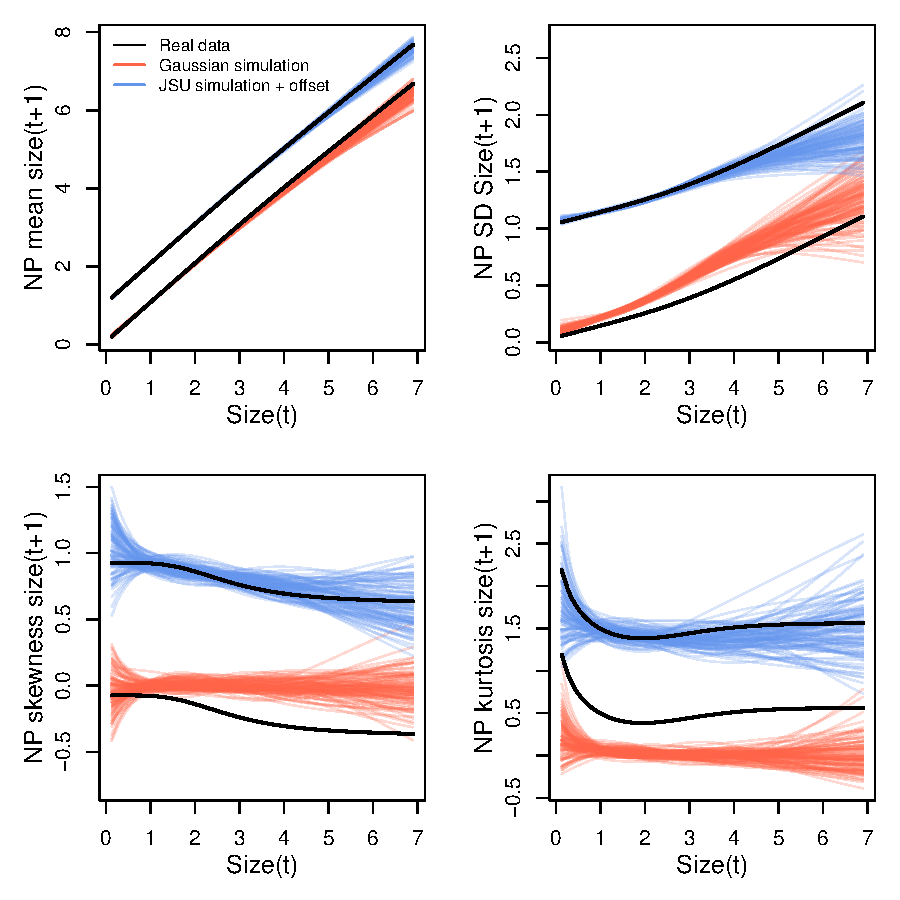
\includegraphics[width=0.75\textwidth]{figures/lichen_JSU_fit}
	\caption{Comparisons among real lichen data and data simulated from Gaussian and JSU growth models for NP mean, NP standard deviation, NP skewness, and NP excess kurtosis of future size conditional on current size. Colored lines show 100 simulated data sets from the fitted Gaussian (red) or JSU (blue) growth models. Thick black line shows the real data. Gaussian and JSU data are offset by one unit and the real data line is duplicated with a one-unit offset for ease of visualization. Figure made by script \texttt{Vuplicida\_IPMs.R}.}
	\label{fig:lichen_fit}
\end{figure} 

\newpage
\begin{figure}[tbp]
	\centering
	\includegraphics[width=0.8\textwidth]{figures/lichen_extinction_risk}
	\caption{Extinction risk estimated from individual-based simulation of IPMs based on Gaussian and Johnson's S-U (JSU) growth distributions. Figure made by script \texttt{Vuplicida\_IPMs.R}.}
	\label{fig:lichen_extinction}
\end{figure} 

\newpage
\begin{figure}[tbp]
	\centering
	\includegraphics[width=1.0\textwidth]{figures/cactus_lambda_years_plots.pdf}
	\caption{Temporal (\textbf{A}) and spatial (\textbf{B}) heterogeneity in fitness for the tree cholla cactus (\textit{Cylindriopuntia imbricata}) predicted by IPMs using Gaussian or SHASH growth models. Figure made by script \texttt{cactus\_growth\_modeling\_qgam.R}.}
	\label{fig:cactus_lambda}
\end{figure}

\newpage
\begin{figure}[tbp]
	\centering
	\includegraphics[width=0.5\textwidth]{figures/orchid_R0.pdf}
	\caption{Orchid life history results from IPMs using Gaussian or skewed $t$ growth models. Lifetime reproductive success ($R_0$) is shown as a function of mean size of flowering. Dashed vertical line shows the observed mean flowering size.}
	\label{fig:orchid_ESS}
\end{figure} 


\end{spacing}

\end{document}